\chapter{基于容器化多终端服务系统架构设计 }\label{chap:service_system}

\section{引言}
% 这一章主要写的就是大背景,边缘设备的空余资源?
% 引言部分要说明目前存着哪些问题
% 需要对空余资源进行管理和利用
% 为何使用去中心化的自组织网络
% 结合微服务特点

本章的内容结构组织如下:第\ref{sec:service_system_related_work}节介绍了一些相关技术的研究工作,包括自治系统的组网技术,微服务架构;第\ref{sec:service_system_design}节介绍了多终端协同服务系统的架构设计,包括引入微服务架构、终端在系统中的身份、系统模块设计等内容;第\ref{sec:service_system_decentralized_network}节提出了多终端协同服务系统的构建方法,包括自治系统的网络选择、自治系统的组网方式、自治系统的管理节点选择等内容;第\ref{sec:service_system_summary}节总结了本章内容。
\section{相关工作}\label{sec:service_system_related_work}
\subsection{自治系统组网技术}



\subsection{微服务架构}
前面加上康威定律和microservice。

在互联网服务行业中,  微服务架构逐渐成为非常流行的架构,在学术界关于微服务架构也同样有一些研究,下面分别从国内研究和国外研究两方面介绍国内外关于微服务架构的研究工作。

\subsubsection{国内研究现状}
国内相关研究文献中对于微服务的研究工作主要集中在利用微服务框架搭建新的服务系统或者将原有的服务系统微服务化,并分析服务系统的功能性需求和非功能性需求,解决微服务化过程中遇到的一些问题。
北京大学的龙新征等人在文献[4]中针对微服务架构中的服务注册、服务发现、负载均衡等常见问题,提出了一种分层的微服务框架,基于这个框架设计并实现了“北京大学校园移动信息服务平台”,为校内师生提供信息服务。同济大学的郭栋等人在文献[5]中设计了一种基于微服务架构构建的云件 PaaS平台,可以在不需要对传统软件做出任何改动的情况下,将软件部署到云端WEB服务器,并通过浏览器以WEB的形式为终端用户提供软件服务。北京交通大学的谭一鸣在文献[6]中对平台化服务框架的功能性需求和非功能性需求进行了分析,设计并实现了使用API网关构建的微服务系统。南京大学的唐文宇在文献[7]中分析了微服务的安全性访问需求,设计并实现了一个安全系统来解决微服务中的第三方应用审核认证及微服务权限访问控制问题。北京交通大学的肖仲垚在文献[8]中分析了业务微服务化过程中对于通信框架的高效简洁高可用等需求,设计并实现了一种微服务通信框架。北京邮电大学的宋鹏威在文献[9]中设计了一个“开放式微服务框架”,并归纳出了一组行业相关开发者在开发过程中所需要注意的内容和原则。作者还基于这些内容和原则完成了一个“开放式数据采集、存储和分析服务” ,证明了该框架对微服务的开发指导工作的有效性。

\subsubsection{国外研究现状}
国外相关研究文献中对于微服务技术的研究工作可以分为4个方面:介绍微服务架构,并结合具体项目来说明效果;开发微服务相关组件或工具,实现微服务架构下的某些特殊功能;评估比较微服务架构的性能;宏观讨论企业从单体式架构转变为微服务架构的原因及可能遇到的问题。

在具体微服务架构项目方面,Hasselbring在文献[10]中介绍了在欧洲最大的电子商务平台之一的otto.de上引入微服务架构,沿业务服务进行垂直分解,为应用和服务提供高可扩展性和高可用性的能力,并解决了微服务化过程中的耦合、集成、可伸缩性、监视和开发等问题。Innerbichler等人在文献[11]中设计并开发了一种基于微服务架构的物联网平台NIMBLE,该平台通过分散,可扩展服务的组合来实现平台的核心业务功能,服务之间以及平台用户、制造商、供应商、传感器和Web资源之间的通信通过简单的协议和轻量级机制来支持。在开发微服务组件方面,Granchelli等人在文献[12]中设计了一种用于微服务体系结构恢复的原型工具MicroART,能够生成基于微服务的系统软件架构模型。Mayer等人在文献[13]中提出了一种用于微服务的监控和管理的实验仪表,能够满足用户不同需求并支持集成不同监控设施来收集微服务运行数据。在评估微服务架构性能方面,Amaral等人在文献[14]中利用主从式和嵌套式容器两种模型来比较微服务架构中的CPU和网络性能。Ueda等人在文献[15]中使用了Acme Air来分析比较微服务和单体架构运行Node.js和Java的性能,实验结果表明相同的硬件配置下微服务的额外开销更大,消耗时间也更多。在宏观讨论企业微服务化可能遇到的问题方面,Kalske等人在文献[16]中指出,迈向微服务架构的典型原因是复杂性、可扩展性和代码所有权,企业微服务化面对的挑战可以分解为技术挑战和组织挑战,前者包括微服务的解耦、划分服务边界代码重构等,后者则包括根据康威定律将大的团队分为可以自主工作的小型团队等等。

\section{多终端协同服务系统架构设计}\label{sec:service_system_design}
\subsection{终端资源特点}
终端资源拥有如下特点:
\begin{itemize}
    \item 终端资源总体数量庞大
    \item 终端资源单体数量较少
    \item 终端之间异构型强
    \item 终端局部网络通信时延小
\end{itemize}

\subsection{微服务架构}
% 说明微服务架构更适合终端服务系统

微服务架构是一种互联网应用服务的软件架构,主要应用于互联网应用服务的服务端软件开发。微服务架构由面向服务架构SOA发展而来,其核心理论基础来自于康威定律[2]中关于组织结构与其设计的系统结构之间关系的描述,即任何组织设计的系统,其结构都是组织本身沟通结构的复制。

2014年学者Martin Fowler正式提出微服务架构的概念[3]:微服务架构以一套微小的服务的方式来开发和部署一个单独的应用,这些微小的服务根据业务功能来划分,通过自动化部署机制独立部署运行在自己的进程中,微服务之间使用轻量级通信机制来进行通信。一个典型的微服务架构应该包括客户端、微服务网关、服务发现、微服务原子层、数据库、部署平台等模块,根据不同应用类型及服务规模,可以增加负载均衡、权限认证、服务熔断、日志监控等模块,来满足服务的非功能性需求。

虽然Martin Fowler给出了微服务的一种定义,但是他也同时指出,微服务并不局限于该定义。Martin尝试归纳和描述微服务架构风格所具有的共同特点,这些特点并不是所有微服务架构风格都要拥有的,也不是用来定义微服务架构本身的,而是微服务架构风格被希望要拥有的特点。也就是说,微服务架构风格不是微服务化的终点,而是微服务化的方向。下面简单介绍一下文献[3]中总结的几个微服务架构风格的特点。

% \begin{itemize}[leftmargin=12pt]
\begin{itemize}
    \item 服务组件化:微服务中,服务可以被当作进程外组件,独立进行部署,服务之间利用网络服务请求或者远程过程调用来进行通信。一个好的微服务架构的目标是通过服务合同中的解耦服务边界和进化机制来帮助各个微服务独立部署运行。微服务架构的设计者希望对任何一个组件或者服务的改动和升级都只需要重新部署该服务而不需要重新部署整个应用程序,并且在升级过程中尽可能少地改变服务间通信的接口。
    \item 围绕业务功能组织服务:当把一个大的应用拆分成小的部分的时候,通常的方法都是根据技术层面分为UI团队、服务端逻辑团队和数据库团队。但是这种拆分团队的方式会使得即使一个简单的变动都会导致整个团队需要耗费时间和预算来适应和协调。康威在文献[2]中提出了康威定律,其中有一条提到:任何组织设计的系统,其结构都是组织本身沟通结构的复制。根据康威定律的这条描述,微服务架构采用围绕业务功能来拆分应用和组织服务的方法。在微服务架构中,设计组织被分为小的开发团队,与之相对应的是,应用被拆分为小的服务,应用之间的沟通过程就是团队之间的沟通过程。为保证应用之间沟通过程清晰明确,团队之间需要划分清晰的服务边界。这样的划分方法也要求每个小团队本身提供开发过程中所需要的所有技能。
    \item 基础设施自动化:许多开发团队都是使用持续交付和持续集成技术来构建微服务架构的应用和系统的,这使得基础设施自动化技术得到了广泛的应用。而随着容器技术、云计算技术等技术在过去几年的快速发展,基础设施自动化技术取得了长足的进步,这也间接降低了微服务构建、部署、运行的复杂性。

\end{itemize}

根据微服务架构的这些特点,我们可以看出,微服务架构非常适合应用到多终端协同服务系统中。对于终端服务来说,终端拥有海量资源,但这些资源以较为分散的、单体资源较少、终端总数量较多、终端之间异构性强的特点分布在终端上面。将微服务架构引入到多终端协同服务系统中来,可以将终端资源的特点与微服务架构的特点很好地结合起来。

对于单体资源有限的终端来说,庞大而复杂的单体式服务应用会消耗大量终端资源,单个终端难以满足其服务的质量。而海量的空闲终端资源分布较为分散,对于维持和提升单体式服务质量也并没有帮助。将单体式服务改编成组件化的微服务后,每个组件式的微服务都只会消耗较少的终端资源,这样分散的终端资源也能够有效维持和提升微服务的质量,另一方面也是提升了终端资源的利用率。微服务架构围绕业务功能组织服务,拆分后的各个小的应用之间通过轻量级通信机制进行数据通信。而终端之间通常通过局域网交换信息,网络传输速度比较快,节点之间距离近,时延较小,相比传统的终端与云端之间进行远距离通信要更加具有实时性,响应速度更快,终端服务质量也更好。微服务架构使用自动化的基础设施,通常利用容器技术来对服务进行部署和构建,与终端服务系统利用容器技术来管理利用终端资源、形成终端资源池、并以容器的形式对外提供服务的特点非常契合。

% \subsection{系统模块设计}
% 整体结构、模块、架构设计图,以及对模块图的说明
% 什么时候进行迁移、对终端资源的利用
% 为什么要使用容器
\subsection{使用容器化}
为了将终端空余资源更好地利用起来,为终端用户提供质量更优的服务,本研究结合终端资源特点,并引入微服务架构的特点,提出了基于容器化的多终端协同服务系统。要将终端上分散的资源利用起来为用户提供服务,使用虚拟化技术是一种很好的方案。虚拟化技术能够将计算机或终端的资源如CPU、内存、存储等抽象、整合起来,打破实体资源的整体性,形成可以按需分配的资源池,让用户能够以更高效合理的方式来对计算机或终端资源进行管理和利用。

虚拟化技术的具体实现形式是虚拟机。虚拟机是一种运行在宿主机上面的,利用虚拟化技术形成的独立的、隔离的虚拟主机,每台虚拟机中可以独立运行属于它自己的不同的操作系统,并在虚拟机内部运行独立的应用程序,从内部运行的应用程序的角度来看,虚拟机就像一台完整的计算机或终端一样,虚拟机的用户、应用程序和虚拟机操作系统不能够分辨虚拟机跟一台物理主机(bare-metal host)之间的区别。由于虚拟化技术的抽象、隔离等特点,多台虚拟机可以同时运行在一台物理主机上,共享宿主机的资源,而且它们彼此之间并不会互相干扰,只会把对方当作另一台独立的计算机或终端主机,运行在虚拟机中的应用程序的安全性更好。另一方面,每台虚拟机都可以从资源池中根据需要配置相应的CPU、内存、存储等资源,相比直接运行在物理主机上,运行在虚拟机中的应用程序的可用性更好。

传统的虚拟机(Virtual Machine,简称为VM)通常使用的是硬件虚拟化技术,在宿主机底层硬件之上独立于操作系统创建了一层虚拟机监视器(Hypervisor),将底层硬件环境进行虚拟化,为上层VM虚拟机的操作系统的运行提供支持。使用VM虚拟机可以为用户提供一个隔离得非常彻底的运行环境。但是VM虚拟机从底层虚拟出一整套操作系统,需要占用非常大的存储空间。而且由于硬件虚拟化技术是处理器密集型技术,会带来大量额外的运行开销,大大加重宿主机的运行负载。这些显然与终端资源的单个终端资源有限的特点有冲突,资源利用率低。另外,VM虚拟机的启动时间非常长,甚至长达几分钟,也非常不适合追求快速响应的终端服务系统。

因为VM虚拟机应用于终端服务系统的资源管理会带来一系列问题,所以我们使用了容器技术来进行终端服务中的资源管理。容器技术是一种轻量级虚拟化技术,是一种操作系统(Operation System,简称为OS)层的虚拟化技术。容器技术可以在宿主机操作系统之上隔离出一个独立的“虚拟机”,这个“虚拟机”通常被称为容器。容器技术底层使用的是基于Linux内核的Linux Container(LXC)技术,而不需要进行额外的虚拟化操作。LXC技术的核心技术包括Namespace技术和Cgroups技术。Namespace技术可以为容器提供一个独立的、隔离的命名空间,其中包含PID(进程)、UTS(host name)、MNT(文件)、NET(网络)、IPC(进程间交互)、USER(用户)等六个方面。不同命名空间的进程彼此之间看不到,Namespace单独隔离出来的命名空间中的容器与其宿主机之间也是彼此看不到,只能通过UTS将对方当作网络中的另一个主机节点,这样就保持了容器的独立性和隔离性。而通过Cgroups技术,可以对每个容器所拥有的CPU、内存、存储、输入输出等资源进行进程级别的管理和配置,这样就使得用户可以利用容器对终端资源进行按需分配管理。同时,利用Cgroups控制组,也能够对对容器内各种资源的消耗情况做监控。因为容器底层仍然是利用宿主机的操作系统,所以相比VM虚拟机,容器技术基本没有太大的额外性能损耗,启动一个容器也相当于启动一个进程,启动时间基本为秒级时间。引入了容器这种轻量级虚拟化技术,我们可以在更为有效地对多终端协同服务系统中的终端资源进行管理和利用的同时,避免了传统VM虚拟机对于终端资源的额外消耗和浪费。

\subsection{层次图}
本研究设计了基于容器化多终端协同服务系统,其层次图如图\ref{fig:system_hierarchy}所示。
\begin{figure}[!htbp]
    \centering
    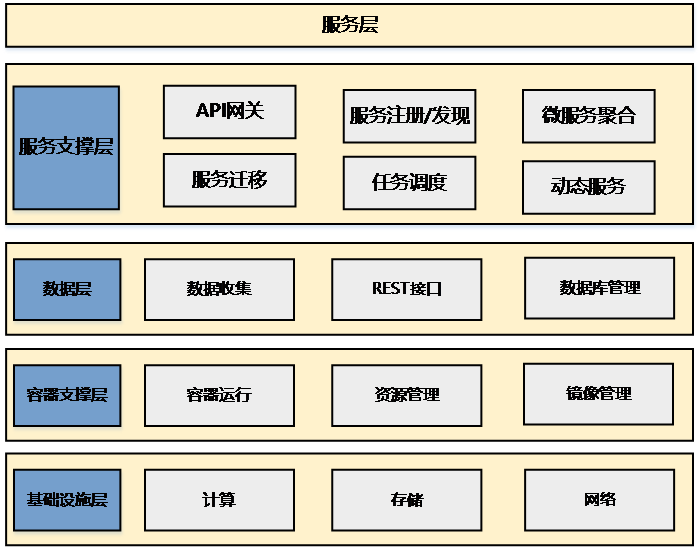
\includegraphics[width=1.0\textwidth]{System_Hierarchy_Chart_Temp}
    \caption{基于容器化多终端协同服务系统层次图}
    \label{fig:system_hierarchy}
\end{figure}

系统最底层为基础设施层,主要为终端设备为上层服务所能提供的资源,包括计算、存储、网络等资源。这些资源为物理实体资源,处于空闲状态,未被组织起来,难以直接向上层服务提供。为了将这些终端物理实体资源组织管理起来,我们在基础设施层上面增加了容器支撑层。这一层中利用容器虚拟化技术,实现容器运行时支撑、容器生命周期管理、容器对底层实体资源的管理、容器内部资源使用情况监控、容器镜像仓库管理等等功能。
% 这里要说一下docker移植的工作,先不加了,后面再说
Docker技术近几年发展迅速,成为容器虚拟化技术的代表,本研究中涉及到的实验及系统设计,均使用Docker技术来代表容器技术。Docker容器技术在终端上部署的架构图如图\ref{fig:docker_architecture}所示。容器支撑层中的容器运行时的具体实现是Docker Container。对容器的生命周期管理主要通过Docker Containerd来实现,具体的生命周期管理工作还包括容器的创建、运行、关闭等。对终端资源的管理和对容器资源的监控主要通过Docker的Cgroups来实现,具体的资源管理工作还包括对终端可用资源的监控和上报、对终端资源进行资源池化、按需划分终端资源、监控本地资源使用情况、当资源利用出现异常时进行报警处理等。对容器镜像仓库的管理主要是通过Docker Image Repository来管理系统内所涉及到的服务的镜像,具体的镜像管理工作还包括镜像的存储、更新、分发下载等。
\begin{figure}[!htbp]
    \centering
    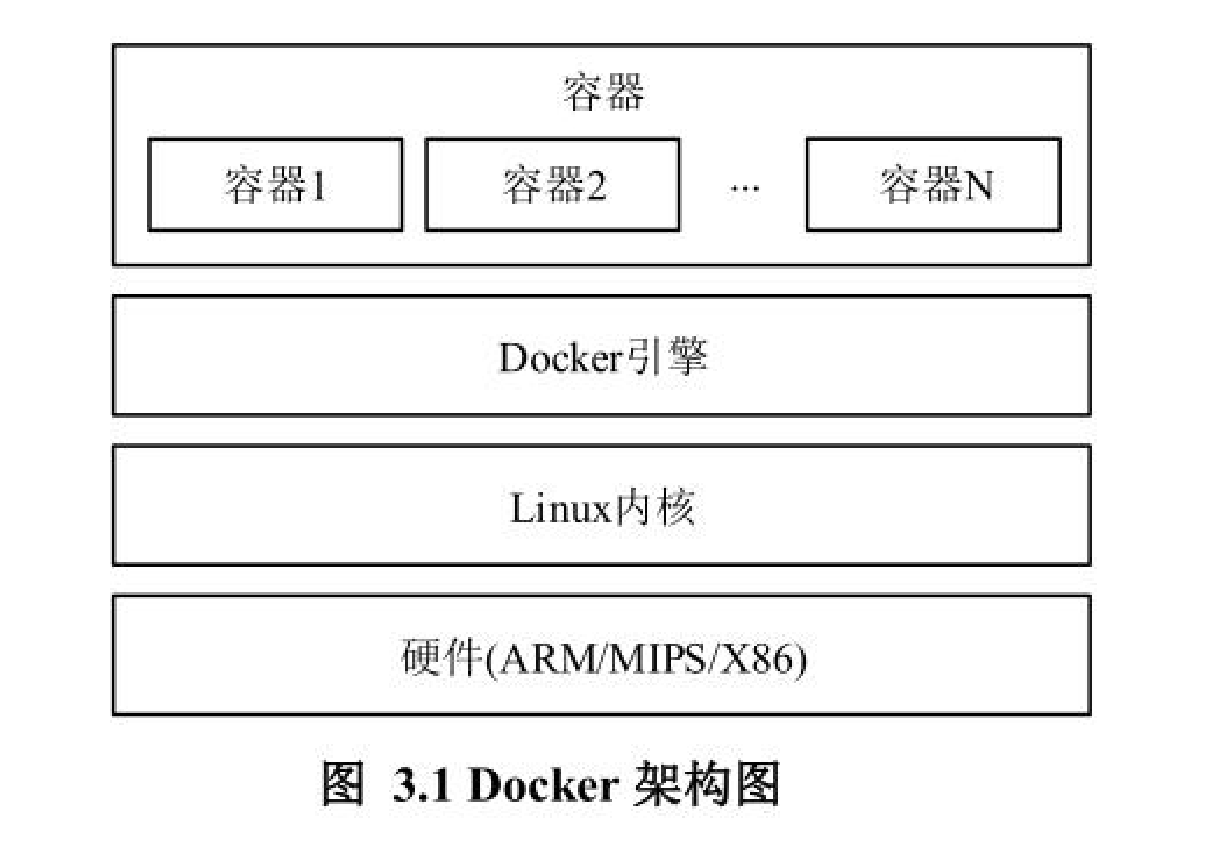
\includegraphics[width=1.0\textwidth]{Docker_Architecture_Temp}
    \caption{Docker容器架构图}
    \label{fig:docker_architecture}
\end{figure}

容器上面一层是数据层,是承上启下的一层。这一层的主要功能是对底层上报的资源数据进行收集整理、为上层微服务之间的通信提供REST接口、对多终端协同服务系统的数据库进行管理等等。数据层上面是服务支撑层,这一层借鉴了很多微服务架构中的模块,主要包括:
\begin{itemize}
    \item API网关:接收用户请求并将其分解为具体的微服务请求
    \item 服务注册:向系统中注册新的可提供的微服务
    \item 微服务聚合:将多个微服务的计算结果整合起来返回给用户
    \item 服务迁移:当出现节点变动的时候,比如节点出现故障下线,或者新节点上线的时候,将服务迁移到其他合适节点上继续运行
    \item 任务调度:根据任务类型及节点资源类型,将任务调度到最合适的终端节点上运行,达到最优调度
    \item 动态服务:根据用户请求流量,动态调整服务规模大小
\end{itemize}

整个系统的最顶层则是服务层,这一层主要包含多终端协同起来为用户提供的各种服务。同时这一端也是更多地交给了终端服务的开发者来实现。终端服务的开发者只需要将开发好的服务应用,通过服务注册模块注册到系统中即可。

\subsection{结构图}
本研究设计的基于容器化多终端协同服务系统,其架构图如图\ref{fig:system_architecture}所示。
\begin{figure}[!htbp]
    \centering
    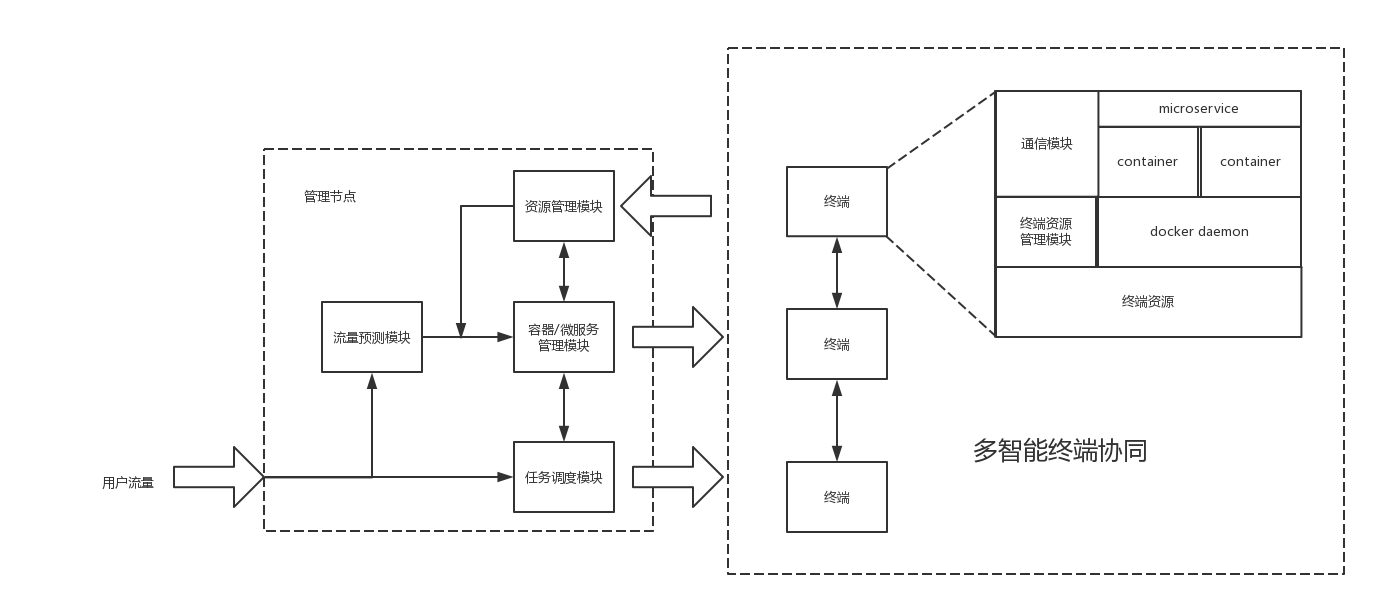
\includegraphics[width=1.0\textwidth]{System_Architecture_Temp}
    \caption{基于容器化多终端协同服务系统架构图}
    \label{fig:system_architecture}
\end{figure}

% 容器与服务管理模块名字要改一下,去掉容器,流量预测模块也改成弹性服务模块
在架构图中,整个系统可以分为管理节点和普通执行节点。在管理节点中包含了弹性模块、资源管理模块、服务管理模块以及任务调度模块。当一个新的终端节点上线的时候,需要向资源管理模块汇报该节点的资源情况,包括可提供资源类型及本地资源负载情况等。当一个新的服务上线的时候,需要向服务管理节点进行注册,向镜像仓库上传镜像,并根据资源管理模块的安排,分配合适的节点运行容器。当用户请求流量到达管理节点的时候,会由任务调度模块进行统一调度,根据服务部署情况及终端节点资源情况选择合适的节点和容器进行执行。另外,当用户请求流量到达管理节点的时候,弹性服务模块会记录该数据,对未来一段时间的用户请求流量情况进行预测,并根据资源管理模块的反馈情况,计算出服务规模的最优大小,由服务管理模块进行服务规模弹性调整。这其中的任务调度模块与弹性服务模块也是本文后面两章的研究重点。

在架构图中,每个终端物理节点代表着层次图中的基础设施层,终端上运行的Docker Daemon和Docker Container代表着层次途中的容器支撑层,管理节点与普通执行节点之间进行的数据交换代表着层次图中的数据层,管理节点中的几个模块代表着层次途中的服务支撑层,终端中运行的微服务应用程序则代表着层次图中的服务层。

\subsection{终端在系统中的角色}

基于容器化多终端协同服务系统中的终端有三个身份,每个终端需要完成终端本身为用户提供的工作,即“本地服务”,当终端本身资源不足不能够很好的完成用户请求的任务,则应该通过系统中的调度中心向其他空闲节点请求提供相应资源来进行协同服务,而当终端本身资源有剩余的时候,该终端又可以通过调度中心将本身的资源以容器虚拟化的形式向系统中的其他节点提供出去。

在这个系统中,用户、服务、终端、容器这几个概念之间的关系如图\ref{fig:system_conception_relationship}所示。用户是整个服务过程的发起者,能够通过自己身边的任何一个设备访问该设备提供的服务,用户对服务的每一次访问都是一次请求任务。服务代表终端能够为用户提供某种服务的能力,是一个比较虚的概念,具体包含两种能力:提供该服务应用的虚拟化容器(或虚拟化镜像)和能够支持该容器快速运行的相应资源。新的服务上线需要向系统注册服务信息,提供服务镜像,上报服务运行所需要的相应资源,并暴露相应服务端口。用户访问服务的过程,实质是用户通过服务对外暴露的端口访问部署在终端上的容器,并由终端向用户提供相应的资源。

\begin{figure}[!htbp]
    \centering
    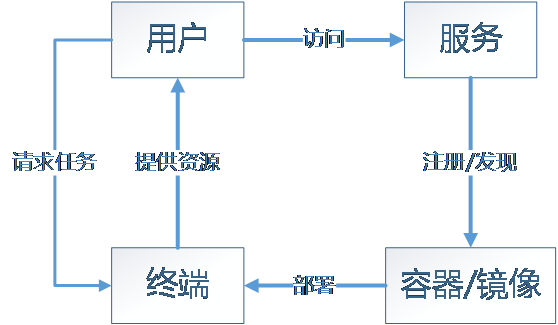
\includegraphics[width=1.0\textwidth]{System_Conception_Relationship_Temp}
    \caption{用户、服务、终端、容器概念之间的关系}
    \label{fig:system_conception_relationship}
\end{figure}


\section{多终端协同服务系统的构建方法}\label{sec:service_system_decentralized_network}
\subsection{自治系统的网络选择}
% 这一节主要说明为什么使用去中心化的网络

自组织网络的应用遍布于军事、数据通信和突发事件处理等领域,其体系结构是指包含协议和拓扑的网络整体设计,拓扑是自组织网络研究中的典型问题。动态条件下建立满足应用的自组织网络是网络体系结构研究的最终目标。自组织网络与现在大部分网络不一样,由于现阶段网络是一种基于客户端-服务器模式下的网络,通过客户端发送请求,利用服务端接收反馈需求,其中各种网络设备在网络中具有特定角色,而自组织网络中的各种设备是对等的。在信息交互时,自组织网络既可以作为客户端,也可做服务端。因为预先建立的基础骨干网设施还不够完善,所以对于终端系统来说,应该使用去中心化的系统架构。

\subsection{去中心化的自组织网络构建}

对于整体而言,利用各个节点间的连接情况来构建一个Connectivity-based Decentralized Node Clustering(CDC)。首先选择若干初始种子节点,初始种子节点的选择算法可以进一步进行研究。每个种子向周围的邻居节点发送消息,消息中会携带ID、种子节点ID、权重、TTL、发送节点相关信息等信息,邻居节点在收到消息后会对该消息做一定处理,并加入节点自身相关的信息,再发送到它的邻居节点。节点消息不断传递下去,直到传递到某个已经确定属于其他集群的节点,或者权重信息消耗尽,或者TTL减小到0,则认为消息传递结束,消息传递过程中经过的节点形成一个集群,集群中的节点互相交换相关信息。在集群内部,可以通过考虑上线时间、稳定程度、负载情况、计算能力、邻居数量、网络状态等信息,选择一个超级节点作为集群的任务调度节点。而当有新的节点上线的时候,不需要重新进行集群的划分,而是应该让该节点向周围邻居节点广播消息,根据网络相关程度、上线时间、地理位置、特殊Tag等方法选择周围邻居节点中的一个加入其所在集群。这样就形成了一个整体去中心化、终端节点自治的一个多终端协同服务系统的底层结构,如图\ref{fig:system_cdc_build}所示是一个简化的模型。
\begin{figure}[!htbp]
    \centering
    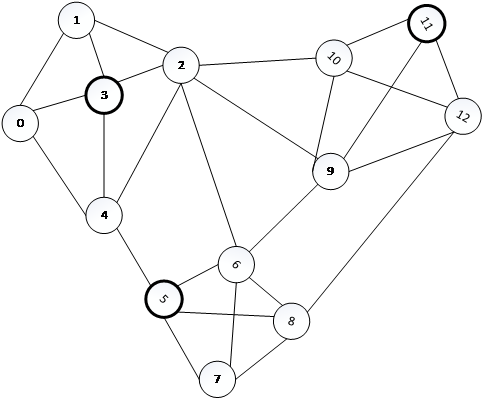
\includegraphics[width=1.0\textwidth]{System_CDC_Build_Temp}
    \caption{去中心化的自组织网络结构}
    \label{fig:system_cdc_build}
\end{figure}
% \subsection{自治系统的管理节点选择}


\section{本章小结}\label{sec:service_system_summary}